%!TEX program = xelatex
% not lualatex because of a pgf bug: https://sourceforge.net/p/pgf/bugs/384/
\documentclass[12pt, a4paper]{report}
\usepackage[T1]{fontenc}
\usepackage[french]{babel}
\usepackage{hyperref}
\usepackage{utbmcovers}
\usepackage{subcaption}
\usepackage{bookmark}
\usepackage{hyphenat}
\usepackage[scale=0.75]{geometry}
\usepackage{overpic}
\usepackage{tikz}
\usepackage{float}

\usetikzlibrary{arrows, positioning}

%----------------------------------------
% hyperref configuration
%----------------------------------------
%
\definecolor{airforceblue}{rgb}{0.36, 0.54, 0.66}

\hypersetup{
    colorlinks=true,
    allcolors=airforceblue,
    urlcolor=airforceblue,
}

\graphicspath{{images/}}

\newcommand\tab[1][1cm]{\hspace*{#1}}
\newcommand\TODO[1]{\textcolor{red}{TODO\@: #1}}

%----------------------------------------
% utbmcovers configuration
%----------------------------------------

\setutbmfrontillustration{monitoring.jpg}
\setutbmtitle{Développement d'un système de video-surveillance à faible latence}
\setutbmsubtitle{Rapport de travail complémentaire \hyp{} A2019}
\setutbmstudent{Nicolas BALLET}
\setutbmstudentdepartment{Département Génie Informatique}
\setutbmstudentpathway{Filière libre}
\setutbmcompany{ }
\setutbmcompanyaddress{ }
\setutbmcompanywebsite{ }
\setutbmcompanytutor{ }
\setutbmschooltutor{Frank Gechter}
\setutbmkeywords{Video surveillance \hyp{} Raspberry pi \hyp{} Gstreamer \hyp{} Github \hyp{} Reconnaissance faciale}
\setutbmabstract{J'ai eu l'occasion en paralléle de mon stage de fin d'étude de concevoir et de commencer à produire une solution de video-surveillance à faible coût, à faible latence et facile à déployer.}

%----------------------------------------
% document
%----------------------------------------

\begin{document}
\makeutbmfrontcover{}
\tableofcontents
\chapter{Introduction}
Quand on parle de vidéo surveillance, ça fait souvent débat...\newline
Mais la surveillance peut être primordiale et nécessaire à la sécurité\newline

Je parle de surveillance privée (chez soi) ou en milieu de type escape game, ou le contrôle doit être instantané en cas de problème ou de risque pour les joueurs, mais aussi de moyen de communication unilatéral en temps réel (et donc faible latence obligatoire).\newline

Au même endroit je veux pouvoir voir un ensemble de caméra regroupées sous forme de groupes.\newline
Aucune solution simple, légère, à faible latence et open source sur le marché.\newline
Faible coût\newline

\section{État de l'Art}
\subsection{Solution existantes}
J'ai commencé par rechercher d'éventuelles solutions déjà existantes ou des outils permettant de mettre mon projet en place simplement et rapidement, voici ce que j'ai pu tester:\newline
\begin{itemize}
    \item Motion, qui est une solution de vidéo surveillance capable de détecter du mouvement dans l'image. Cette solution est très simple à utiliser et possède même une distribution GNU/Linux dédiée (MotionEye). Bien qu'il soit paramétrable et permette de modifier la qualité et le nombre d'images par secondes, il implique tout de même une latence non négligeable.\newline

    \item Quelques forums ont aussi mentionnés l'utilisation de la librairie Python picamera, qui permet de récupérer le flux de la camera d'une raspberry pi et de le servir via une page web. Cette solution, bien que rapide à mettre en place, n'offre pas des temps de réponses acceptables.\newline
        \url{https://raw.githubusercontent.com/RuiSantosdotme/Random-Nerd-Tutorials/master/Projects/rpi_camera_surveillance_system.py}\newline

    \item Vlc, logiciel de lecture vidéo très polyvalent, permet aussi de faire du streaming vidéo. Cette solution, implique aussi une certaine latence.\newline

    \item Ffmpeg, programme de traitement de flux audio et vidéo offre la possibilité de servir un flux vidéo en streaming mais encore une fois, impliquant une trop grande latence et un nombre d'images par secondes trop bas.\newline

    \item{J'ai aussi pu essayer Gstreamer qui est une librairie de manipulation de flux vidéo et audio reposant sur l'utilisation de pipelines. Deux configurations ont attirés mon attention:\newline
        \begin{itemize}
            \item D'une application Gstreamer à une autre application Gstreamer, offrant de très bonnes performances, mais peu pratique, car implique d'installer l'application cliente afin de recevoir le flux.\newline
            \item D'une application Gstreamer App vers un navigateur web, offre encore une fois de très hautes performances, le seul point négatif est que je n'ai pu trouver sur internet qu'une preuve de concept utilisant cette méthode.\newline
        \end{itemize}
        }
\end{itemize}
\TODO{Inserer images de comparaison des latences}\newline
J'ai choisi d'utiliser Gstreamer pour ses performances et la modularité qu'offre son système de pipeline.\newline

\subsection{Langage d'implémentation}
Cette librairie peut être utilisée dans de multiples langages, j'ai du faire un choix parmi ceux que j'avais déjà utilisés auparavant.\newline
\begin{itemize}
    \item Le C, langage bas niveau et performant. C'est avec ce langage que la preuve de concept qui m'a servie de référence à été implémentée.\newline
    \item Le C++ aussi performant mais dont le cout de développement est plus faible car il offre un plus haut niveau d'abstraction, mais aussi car il offre un meilleur contrôle de la mémoire.\newline
    \item Et le Python, moins performant mais plus facile à utiliser.\newline
\end{itemize}
\begin{figure}[H]
    \begin{minipage}{.5\textwidth}
        \centering
        
\includegraphics[width=.5\textwidth]{c.png}
        \caption{Logo du langage de programmation C}
    \end{minipage}
    \begin{minipage}{.5\textwidth}
        \centering
        
\includegraphics[width=.5\textwidth]{cpp.png}
        \caption{Logo du langage de programmation C++}
    \end{minipage}
\end{figure}
\begin{figure}[H]
    \centering
    
\includegraphics[width=.35\textwidth]{python.png}
    \caption{Logo du langage de programmation Python}
\end{figure}

\subsection{Protocole réseau}
Il existe beaucoup de protocoles réseau afin de streamer un flux vidéo, les plus pertinents sont les suivants:\newline
\begin{itemize}
    \item RTP, une utilisation simple et est supporté par beaucoup de logiciels, notamment Nginx, mais engendre de la latence\newline
    \item WebRTC, nécessite d'implémenter son propre protocole métier via des WebSockets, mais apporte une très faible latence\newline
\end{itemize}
\begin{figure}[H]
    \centering
    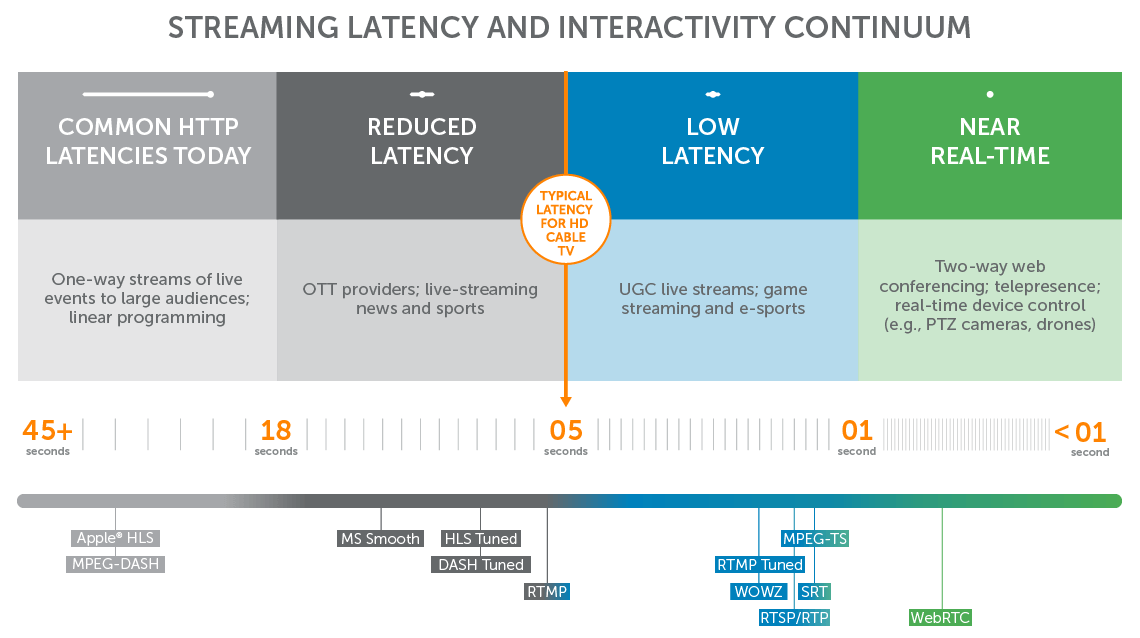
\includegraphics[width=1.0\textwidth]{realtime-protocols.png}
    \caption{Graphique de synthèse des latences par protocole}
\end{figure}

\subsection{Encodage vidéo}
L'encodage se devant d'être compatibles avec les navigateurs récents, la liste est assez courte:\newline
\begin{itemize}
    \item H264, performant, encodage matériel sur les raspberry pi 2 et 3\newline
    \item VP8/VP9, moderne, performant, utilise moins de bande passante, mais les raspberry pi 2 et 3 ne comporte pas l'encodage matériel nécessaire, ce qui les rendent inutilisables sur mon matériel\newline
\end{itemize}
\begin{figure}[H]
    \begin{minipage}{.5\textwidth}
        \centering
        
\includegraphics[width=\textwidth]{vp8.png}
        \caption{Logo de l'encodage VP8}
    \end{minipage}
    \begin{minipage}{.5\textwidth}
        \centering
        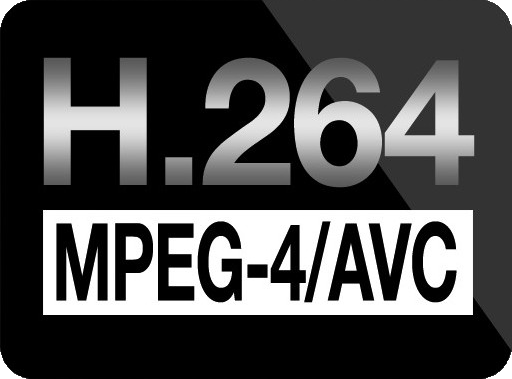
\includegraphics[width=\textwidth]{h264.png}
        \caption{Logo de l'encodage H264}
    \end{minipage}
\end{figure}

\subsection{Technologie serveur}
Afin de centraliser les connexions et potentiellement pouvoir simplement ajouter de l'authentification à postériori, j'ai choisi d'utiliser une structure réseau en étoile avec un serveur central.\newline
La plupart des exemples d'échanges en WebRTC que j'ai pu trouver se trouvaient être implémentés avec un serveur central en Python.\newline
Ici, j'ai choisi d'utiliser Django, qui est un framework d'application web en Python, car il offre beaucoup d'outils et de modules et cela réduit considérablement la charge de travail. L'ayant déjà utilisé sur de multiples projets, le choix était pour moi évident.\newline
Afin de stocker les données j'ai garder le systèmes de base de données par défaut de Django, SQLite. Il ne nécessite aucune configuration et fonctionne directement.

\section{Outils}
\TODO{Neovim}

\section{Définition du sujet}
J'ai donc choisi de me lancer dans le développement d'une solution de vidéo surveillance utilisant Gstreamer, du WebRTC, encodé en H264 (mais paramétrable car dépendant du matériel à disposition). La partie camera en C++ et la partie web en HTML/CSS/Javascript.\newline
Le tout configuré en étoile avec un serveur au milieu, qui servira aussi la page web aux navigateurs. Ce serveur sera implémenté en Python car ne requiert pas de performances.\newline
La solution devra être performante autant en terme d'images par secondes (minimum 15fps) qu'en terme de latence (moins de 1s).\newline

\chapter{Réalisation}
\section{Développement de la caméra}
\subsection{Analyse}
Suite à cette recherche de solutions et de technologies, j'ai commencé par étudier la preuve de concept Gstreamer comportant l'envoi du flux vidéo à un client WebRTC que j'avais trouvé durant mes recherches.\newline
L'établissement d'un connexion WebRTC nécessite plusieurs éléments:
\begin{itemize}
    \item Un accord SDP, définissant le format du flux qui sera échangé
    \item Un accord ICE, définissant la route que le flux empruntera. Cela peut être utile dans le cas d'un proxy séparant la caméra et le client.
\end{itemize}
\subsection{Refonte C++}
Afin de pouvoir utiliser des outils plus haut niveau, j'ai ensuite refondu cette preuve de concept en C++.\newline
Je n'ai pas beaucoup changé la structure du code, ça sera l'objet d'une prochaine refonte.

Quand la caméra démarre, elle met en place la racine de la pipeline et stream le flux vers un "trou noir" (un noeud qui ne fait qu'absorber le flux). Avant ce "trou noir" ce trouve un "tee" qui va permettre de dupliquer le flux et l'envoyer à plusieurs noeuds. C'est ici que les clients WebRTC viendront se brancher une fois que la connexion WebRTC à été négociée.

\TODO{Représentation pipeline}

\section{Développement du serveur}
\subsection{Conception de la base de données}
Les utilisateurs devant pouvoir regrouper les caméras par pièce, j'ai modélisé la base de données qui sera utilisée par le serveur central.
\TODO{Schéma de Base de données}

\subsection{Définition du protocole métier}
Une fois la base de données mise en place, j'ai ensuite développé la logique qui permet aux caméras et aux clients d'échanger des messages et de pouvoir établir des connexions WebRTC.\newline
Les connexions au serveur se font via des WebSockets, cela permet aux clients et aux caméras de générer des événements en temps réel.\newline
Cela rend par contre le système entièrement asynchrone et complexifie l'ensemble des processus.\newline


Un message à cette forme:\newline
\{\newline
    command: 'COMMAND',\newline
    identifier: '0123456789',\newline
    [...]\newline
\}\newline

Quand un message est envoyé, le champ 'identifier' représente le destinataire du message. Il est utilisé par le serveur central afin de savoir à quelle WebSocket il doit transmettre le message. Le serveur remplace aussi la valeur du champ par l'identifiant de la source du message de manière à ce que le destinataire sache de qui vient le message.\newline

Voici la liste des commandes que j'ai implémenté:\newline
\begin{itemize}
    \item JOIN\textunderscore CLIENT\newline
        Utilisé par un client afin de s'enregistrer auprès du serveur.\newline

    \item JOINED\textunderscore CLIENT\newline
        Le serveur répondra ensuite avec un identifiant qu'il aura attribué au client.\newline

    \item JOIN\textunderscore CAMERA\newline
        Utilisé par une camera afin de s'enregistrer.
        Il joindra à la commande, un identifiant que l'administrateur lui aura attribué.
        Par exemple son adresse mac peut-être utilisée afin de pouvoir réinstaller la camera librement sans perdre sa configuration (association caméra <-> pièce).\newline

    \item JOINED\textunderscore CAMERA\newline
        Le serveur répondra ensuite afin de valider la connexion.\newline

    \item CALL\newline
        Un client peut demander à initialiser une connexion avec une camera via cette commande\newline

    \item CAMERA\textunderscore UPDATE\newline
        Quand une camera démarre, elle va envoyé cette commande au serveur central afin qu'il notifie tous les clients connectés qu'une nouvelle camera est disponible. À la suite de quoi ils pourront envoyer une commande CALL.\newline
\end{itemize}
On entre ici dans la partie technique nécessaire au WebRTC\newline
\begin{itemize}
    \item SDP\textunderscore OFFER et ICE\textunderscore CANDIDATE\newline
        Quand la caméra recois une commande CALL, elle va envoyer au client des offres SDP et des offres ICE, afin de négocier respectivement le format du flux et la route à emprunter.\newline

    \item SDP\textunderscore ANSWER et ICE\textunderscore ANSWER\newline
        Après avoir reçu les offres, le client va choisir quelle offre il préfère et va en renvoyer une de chaque type.\newline
        Quand la caméra recevra ces commandes, les clients WebRTC pourront être configurés et le flux pourra être streamé.

\end{itemize}

\chapter{Résultats}
En définitive, le projet est fonctionnel et même très performant.\newline
Il reste des bugs bloquants à résoudre avant de pouvoir être utilisé en situation réelle.\newline
Il n'est pour l'instant pas possible d'afficher plus d'une camera à la fois et les caméras doivent être démarrées après le chargement de la page web. Le premier bug est du à mon implémentation, tandis que pour le second, je soupçonne l'implémentation du module WebRTC d'être défaillante.\newline
J'ai eu de l'aide de la part d'un ami et collègue qui a pu tester ma solution sur d'autres modèles de micro-ordinateurs que ceux que j'avais à ma disposition et me faire des retours de bugs me permettant de stabiliser l'application et la rendre plus polyvalente. Comme par exemple en ajouter la possibilité de customiser la pipeline afin de s'adapter au matériel.\newline
Ce projet était vraiment très agréable à développer. J'aimerais continuer à le développer afin de pouvoir un jour le packager et le proposer à un plus large public.\newline

J'aurais aimé trouver plus de documentation concernant le protocole WebRTC qui n'a pas été facile à utiliser.

J'ai tout de même réussi à afficher un flux vidéo provenant d'une Raspberry pi 3 sur une page web avec une latence avoisinant les 10ms à 30 images par seconde.
\end{document}
